\documentclass[14pt]{extarticle}

\usepackage[margin=0.5in]{geometry}
\usepackage{amsmath}
\usepackage[none]{hyphenat}
\usepackage{pgfplots}
\usepackage{amssymb}
\usepackage{amsmath}
\usepackage{multicol}
\usepackage{tikz}
\usepackage{tikz-3dplot}
\usetikzlibrary{angles, quotes}

\pgfplotsset{compat=newest}

\title{EE-220 Homework 11}
\author{Jonathan Forhan}
\date{ }

\renewcommand{\thesubsection}{\thesection-\alph{subsection}}

\begin{document}

\maketitle

\boldmath
\section{Consider a triangle with vectors $\vec{A}$ and $\vec{B}$ defining
  its two sides and the angle $\theta$ between them.}
\unboldmath

\begin{center}
	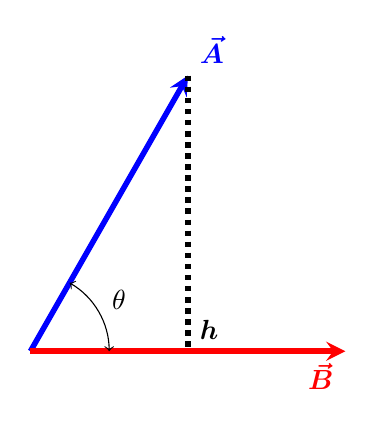
\begin{tikzpicture}
		\coordinate (O) at (0,0);
		% vecs
		\draw[line width=2pt,blue,-stealth] (0,0) -- coordinate (A) (2,3.5) node[anchor=south west]{$\boldsymbol{\vec{A}}$};
		\draw[line width=2pt,red,-stealth] (0,0) -- coordinate (B) (4,0) node[anchor=north east]{$\boldsymbol{\vec{B}}$};
		% dotted
		\draw[dotted, line width = 2pt] (2,3.5) -- coordinate (h) (2,0) node[anchor=south west]{$\boldsymbol{h}$};
		% angles
		\path (A)--(O)--(B)
		pic["$\theta$",draw=black,<->,angle eccentricity=1.3,angle radius=1cm] {angle=B--O--A};
	\end{tikzpicture}
\end{center}

\boldmath
\subsection{Prove that the area of the triangle can be calculated as:
	$S=\frac12|\vec{A}\times\vec{B}|$}
\unboldmath

$$S=\frac12 bh$$
\begin{align*}
	 & \sin\left(\theta\right)=\frac{\textrm{opposite}}{\textrm{hypotenuse}}=\frac{h}{|\vec{A}|}\Rightarrow h=|\vec{A}|\sin\left(\theta\right) \\
	 & \textrm{let $|\vec{B}|$ = b}                                                                                                            \\
	 & h=|\vec{A}|\sin\left(\theta\right)                                                                                                      \\
	 & S=\frac12bh \Rightarrow S=\frac12 |A||B|\sin(\theta)                                                                                    \\
	 & S=\frac12|\vec{A}\times\vec{B}|
\end{align*}

\boldmath
\subsection{Show the triangle defined by the corner points $P(1, 1, 0)$,
	$Q(2, 5, 0)$, and $R(0, 4, 6)$ in the Cartesian coordinates.}
\unboldmath

\begin{center}
	\tdplotsetmaincoords{70}{110}
	\begin{tikzpicture}[scale=1,tdplot_main_coords]
		\draw[thick,->] (0,0,0) -- (7,0,0) node[anchor=north east]{$x$};
		\draw[thick,->] (0,0,0) -- (0,7,0) node[anchor=north west]{$y$};
		\draw[thick,->] (0,0,0) -- (0,0,7) node[anchor=south]{$z$};
		\filldraw[draw=red, fill=red!20]
		(1,1,0)
		-- (2,5,0) node[anchor=north west]{$Q(2,5,0)$}
		-- (0,4,6) node[anchor=south]{$R(0,4,6)$}
		-- cycle node[anchor=north]{$P(1,1,0)$};
	\end{tikzpicture}
\end{center}

\boldmath
\subsection{Calculate the area of the triangle defined in (b) using the equation in (a).}
\unboldmath

\begin{align*}
	S                    & =\frac12 |\overrightarrow{PR}\times\overrightarrow{PQ}|                     \\
	\overrightarrow{PR}  & =\vec{R} - \vec{P} = -\vec{a}_x+3\vec{a}_y+6\vec{a}_z                       \\
	\overrightarrow{PQ}  & =\vec{Q} - \vec{P} = \vec{a}_x+4\vec{a}_y                                   \\
	\overrightarrow{PR}  & \times \overrightarrow{PQ} = (0-24)\vec{a}_x-(0-6)\vec{a}_y+(-4-3)\vec{a}_z \\
	\overrightarrow{PR}  & \times \overrightarrow{PQ} = -24\vec{a}_x+6\vec{a}_y-7\vec{a}_z             \\
	|\overrightarrow{PR} & \times \overrightarrow{PQ}| = \sqrt{24^2+6^2+7^2}=25.71                     \\
	S                    & = \frac12 25.71 = 12.85
\end{align*}

\boldmath
\section{An infinitely long line of current along the z-axis
  has the current $I=2\mathrm{A}$ in the $\vec{a}_z$ direction.}
\unboldmath

\boldmath
\subsection{Find the magnetic field $\vec{H}$ at the point $P(0,4,0)$, created
	by the segment of the line that extends from \\
	$z=0$ to $z=5\mathrm{m}$.}
\unboldmath

\begin{align*}
	\overrightarrow{dH} & =\frac{I\overrightarrow{dL}\times\vec{a}_R}{4\pi R^2}                                             \\
	\overrightarrow{dH} & =\frac{I\cdot dz\vec{a}_z\times(-z\vec{a}_z+\rho\vec{a}_\rho)}{4\pi (z^2+\rho^2)^\frac32}         \\
	\vec{H}             & =\int^5_0\frac{I\cdot dz\vec{a}_z\times(-z\vec{a}_z+\rho\vec{a}_\rho)}{4\pi (z^2+\rho^2)^\frac32} \\
	\vec{H}             & =\frac{I\cdot\rho\vec{a}_\phi}{4\pi}\int^5_0\frac{dz}{(z^2+\rho^2)^\frac32}                       \\
	\vec{H}             & =\frac{2\vec{a}_\phi}{\pi}\int^5_0\frac{dz}{(z^2+16)^\frac32}                                     \\
	\vec{H}             & =\frac{2\vec{a}_\phi}{\pi}\int^5_0\frac{dz}{(z^2+16)^\frac32}                                     \\
	\vec{H}             & =\frac{z}{8\pi\sqrt{z^2+16}}\bigg|^5_0                                                            \\
	\vec{H}             & =0.0311\vec{a}_\phi\mathrm{[A/m]}
\end{align*}

\boldmath
\subsection{Calculate the field created by the segment described in (a)
	at the origin.}
\unboldmath

\begin{align*}
	\overrightarrow{dH} & =\frac{I\overrightarrow{dL}\times\vec{a}_R}{4\pi R^2}                     \\
	\overrightarrow{dH} & =\frac{I\cdot dz\vec{a}_z\times(-z\vec{a}_z)}{4\pi (z^2+\rho^2)^\frac32}  \\
	\vec{H}             & =\int^5_0\frac{I\cdot dz\vec{a}_z\times(-z\vec{a}_z)}{4\pi (z^2)^\frac32} \\
	\vec{H}             & =0\mathrm{[A/m]}
\end{align*}

\boldmath
\subsection{Find the field created at point $P(0,4,0)$ by the segment
	that extends from $z=0$ to $z=\infty$.}
\unboldmath

\begin{align*}
	\vec{H} & =\frac{I}{4\pi\rho}\vec{a}_\phi   \\
	\vec{H} & =0.0398\vec{a}_\phi\mathrm{[A/m]}
\end{align*}

\boldmath
\subsection{Find the field created at point $P(0,4,0)$ by the whole line.}
\unboldmath

\begin{align*}
	\vec{H} & =\frac{I}{2\pi\rho}\vec{a}_\phi   \\
	\vec{H} & =0.0796\vec{a}_\phi\mathrm{[A/m]}
\end{align*}

\end{document}
